\section{Description of the architecture}
\label{sec:description_of_the_architecture}

To analyze the frequency generator designed for this project, we can start from the structure of three main blocks

\begin{itemize}
        
    \item \textbf{Human-Machine interface} \newline
    To select the desired output wave at the right frequency, this generator provides an LCD screen and a keypad. \\
    The keypad is used to write the frequency manually and to select the output waveform, information that is shown on the LCD screen.

    \item \textbf{Digital waveform generator} \newline
    The digital waveform generator uses the DDFS technique to create the digital output. \\
    The representation of the output value is C1 to be compatible with the DAC, and to increase the number of waveforms available, vertical and horizontal mirroring is selectable.

    \item \textbf{Digital analog converter} \newline
    The DDFS module is designed to have a \(12 \ bit\) output digital value, but for the project a is used a VGA DAC that has three \(10 \ bit\) channels. \\
    Only the most significant bits of the module have been used.

        
\end{itemize}

\subsection{Specifications}

The frequency generator designed is capable to generate three different output wave and the mirroring combinations of them, with a total of 8 valid combinations (some combinations are valid but not useful)

\begin{itemize}

    \item \textbf{Square wave} \\
    available only with vertical and horizontal mirroring enabled, for every other combinations of vertical and horizontal mirroring the output value is constant at \texttt{0xFFF} (hex notation), or result in a square wave with two time the selected frequency.
    
    \item \textbf{Triangular wave} \\
    available with vertical and horizontal mirroring enabled.
    If the vertical and the horizontal mirroring is disabled the output is a \textbf{sawtooth wave},
    instead if only the horizontal mirroring is enabled, the output is an \textbf{alternating symmetrical sawtooth wave}
    
    \item \textbf{Sinusoidal wave} \\
    available with vertical and horizontal mirroring enabled.
    If only the vertical mirroring is enabled the waveform is a \textbf{rectified sinusoidal wave}.
    If only the horizontal mirroring is enabled the waveform is an \textbf{alternating symmetrical quarter-sine wave}.
    If both of the mirroring are disabled the waveform is a \textbf{quarter-sine wave}
    
\end{itemize}

\noindent
The output frequency can be selected with an LCD screen and a keypad and can go from \(1Hz\) to \(1MHz\) without using external memory for the LUT.

\vspace{0.5cm}
\[
    max(f_{out}) = \frac{max(f_{clk})}{\texttt{LUT\_DIM}/max(f_w) \cdot 4} = \frac{35MHz}{2^{10}/2^7 \cdot 4} \simeq 1.09MHz
\]
\vspace{0.5cm}

\noindent
The DAC used is a \(10 \ bit\) VGA DAC with three channels synchronized with a common clock at the maximum frequency of \(100 \ MHz\). \\
The maximum clock frequency is \(35MHz\) because the project is synchronized with a common clock source at a frequency of \(70MHz\) that passes through a frequency divider, which dynamically divides the frequency with a division coefficient ranging from \(2\) to \(1000000\).

\newpage

\subsection{Module description}

As seen in the image below, the project is made of different modules 

\begin{figure}[h!]
    \centering
    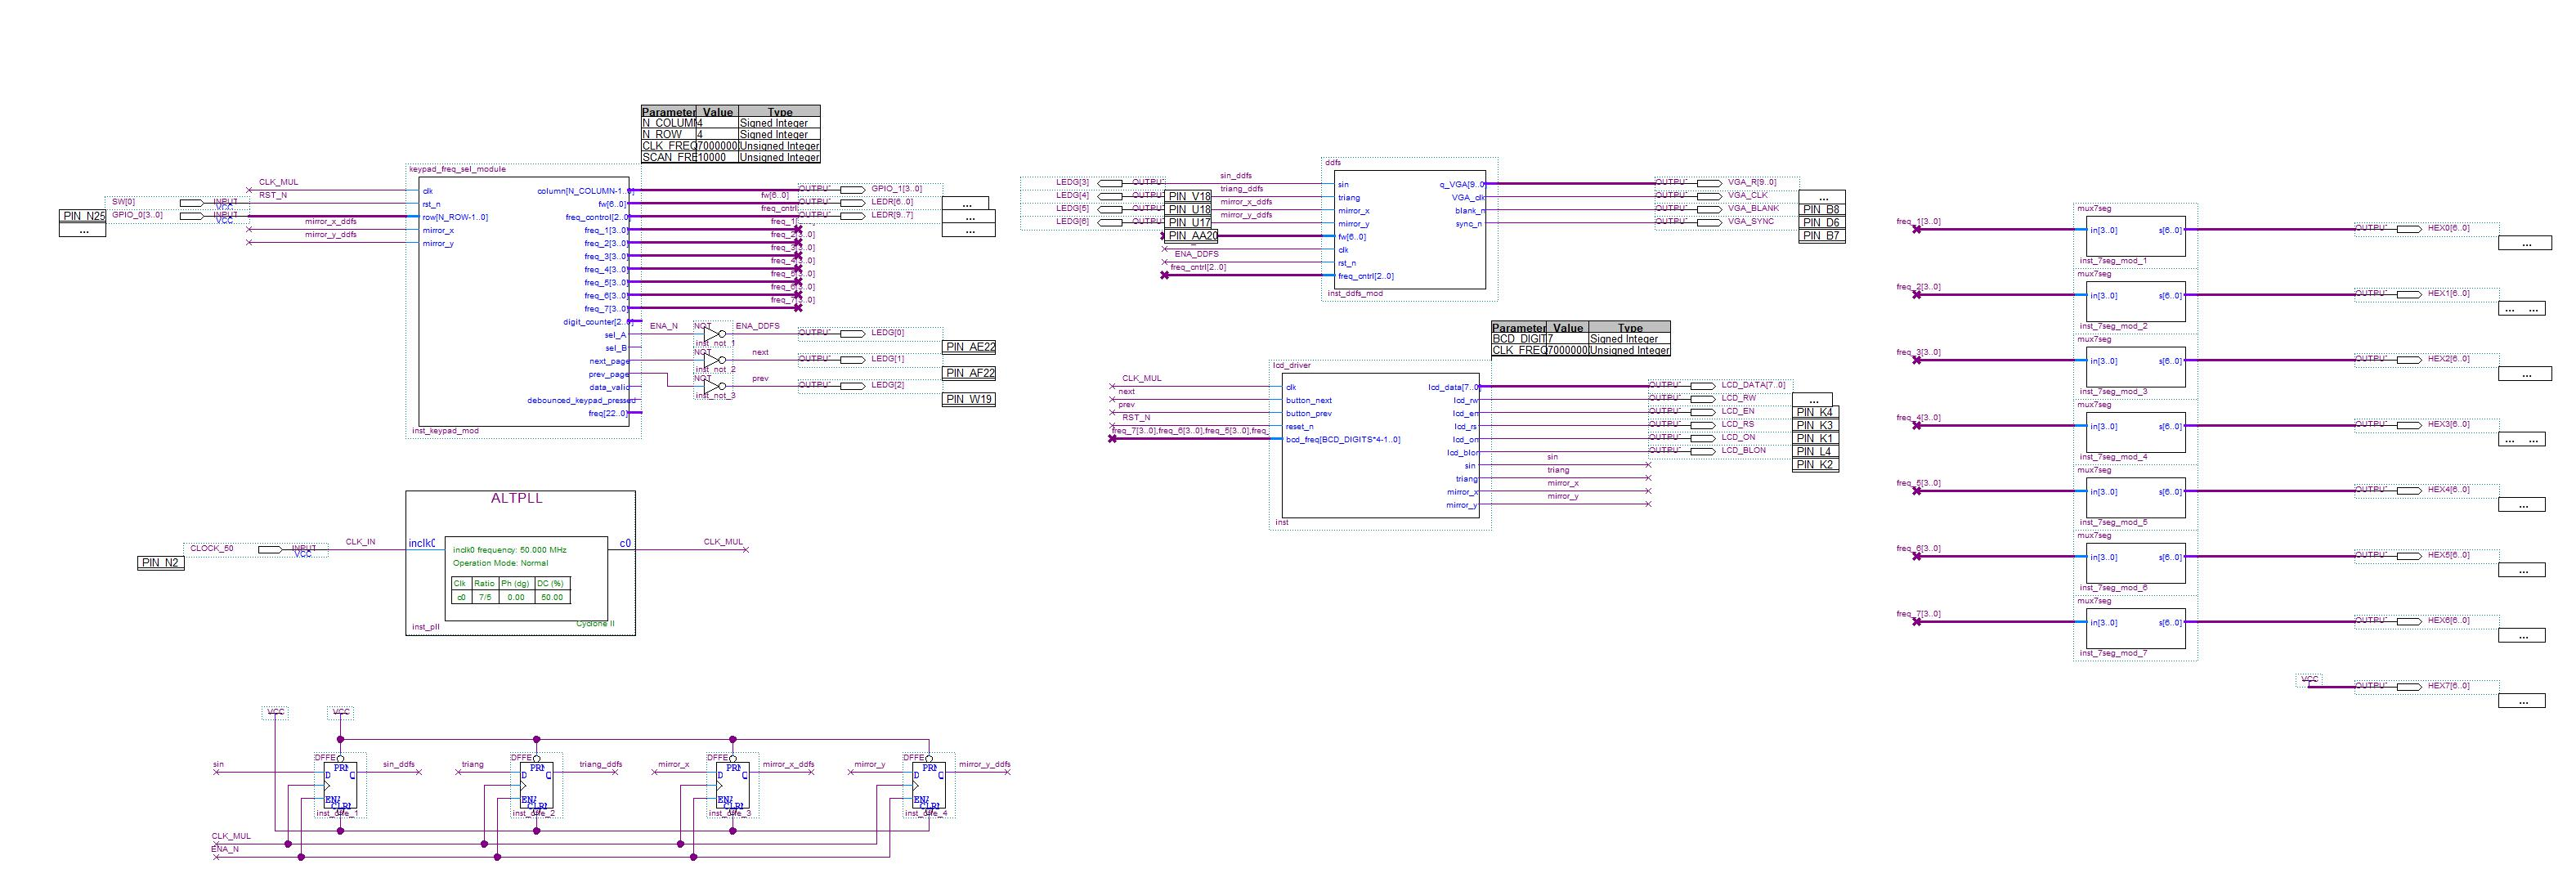
\includegraphics[width=\textwidth]{img/main_function_generator.jpg}
    \caption{Top level entity symbol schematic}
    \label{fig:Top_level_entity}
\end{figure}

\subsubsection{DDFS module}

The DDFS module generates the bit-stream corresponding to the samples of the output waveform at the desired frequency. \\
The samples are synchronized with a common clock signal, and the frequency of the output wave can be selected through the \texttt{fw} and \texttt{freq\_ctrl} inputs. \\
This module has been designed in two different ways:

\begin{itemize}
    \item the first version is intended to be connected to the \textbf{ADV7123 DAC}, which is a \(10 bit\) synchronous VGA DAC
    \item the second version is intended to be connected to a \(12 bit\) asynchronous R-2R ladder DAC.
\end{itemize}

\vspace*{0.5cm}
\begin{figure}[h!]
    \centering
    % Immagine a sinistra
    \begin{minipage}{0.45\textwidth}
        \centering
        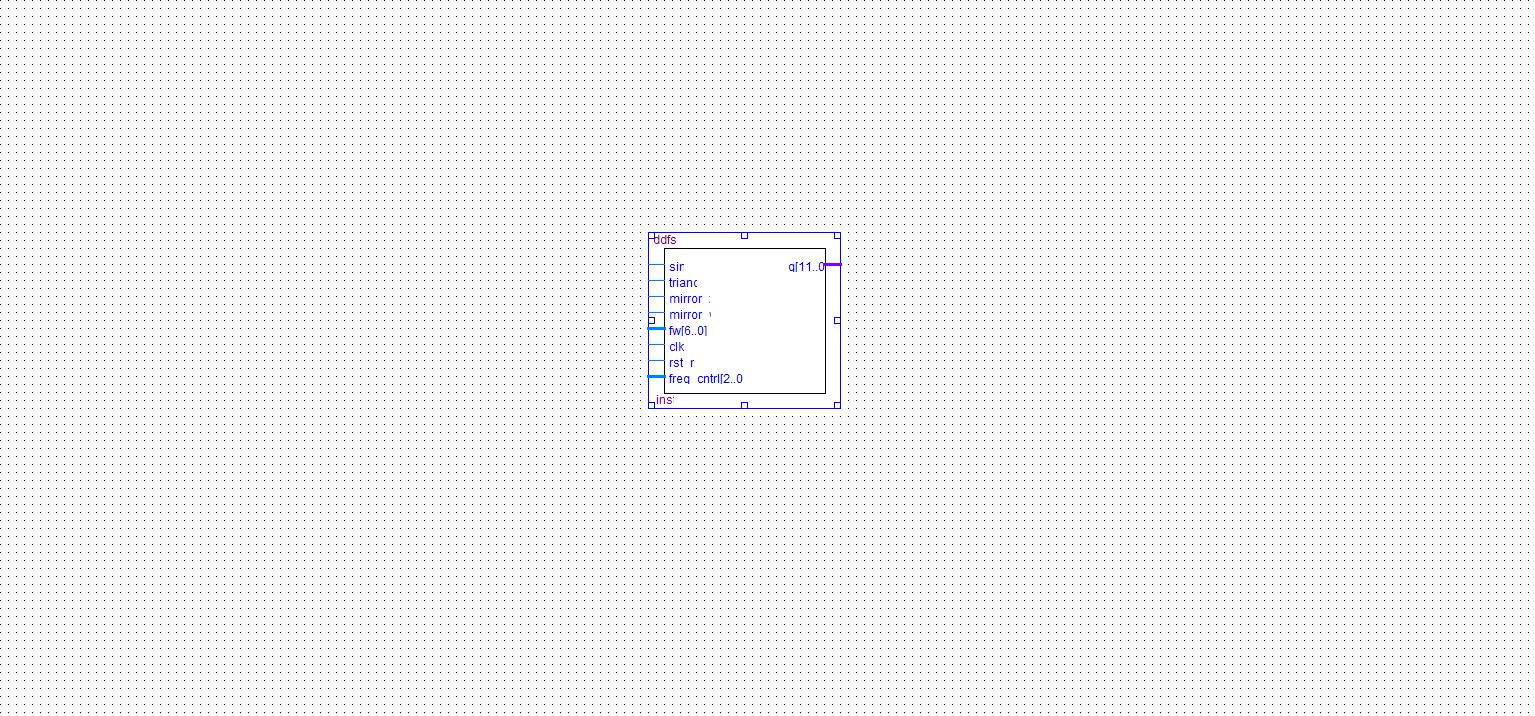
\includegraphics[width=\textwidth, trim={12cm 5.5cm 13cm 4cm}, clip]{img/DDFS_12bit.jpg}
    \end{minipage}
    \hfill
    % Immagine a destra (uguale)
    \begin{minipage}{0.45\textwidth}
        \centering
        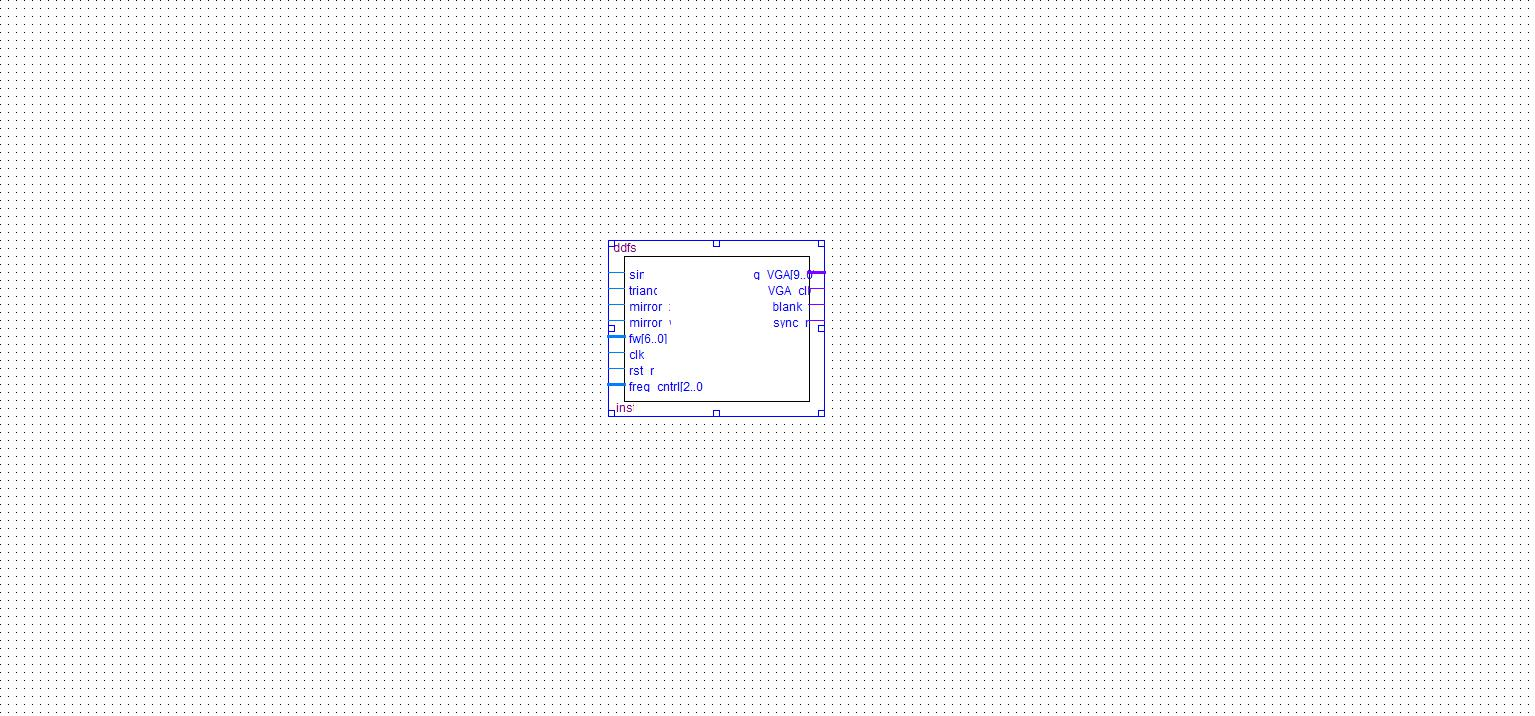
\includegraphics[width=\textwidth, trim={11.5cm 5cm 13cm 4cm}, clip]{img/DDFS_VGA.jpg}
    \end{minipage}

    \caption{DDFS module}
    \label{fig:DDFS_module}
\end{figure}
\vspace*{0.5cm}

\paragraph{I/O interface} \quad \\
The ports used to connect this module to other modules or to the external pins of the FPGA are the following:

\begin{itemize}

    \item \texttt{sin, tri} \\
    used to select the output waveform. If \texttt{sin} and \texttt{tri} are both zero, the output signal is a square wave. The sinusoidal output has priority.
    
    \item \texttt{mirror\_x, mirror\_y} \\
    used to manually select the symmetry of the output wave. \texttt{mirror\_x} is used to enable the horizontal symmetry of the wave, and \texttt{mirror\_y} to enable the vertical symmetry. For every symmetry pin enabled, the period of the output wave doubles because the wave needs to be repeated mirrored.
    
    \item \texttt{f\_w} \\
    is the value of the frequency word. It is composed of \(7bits\) and is 
    \texttt{unsigned}, so the maximum value is \(2^7 - 1 = 127\). The instantiated LUT is a \((12 \ \text{x} \ 1024)bit\) memory where the address value goes from \(0\) to \(1023\), and the stored samples are \(12bit\) values. The number of samples sent to the DAC after a complete scan cycle are \( 8 < \frac{1024}{\texttt{f\_w} + 1} < 1024 \).
    
    \item \texttt{clk, rst\_n} \\
    are the clock and the synchronous reset pins.
    
    \item \texttt{freq\_cntrl} \\
    is a select input used to scale the clock frequency by a fixed value.
    It is a \(3bit\) input pin, and the scalable frequency values are \(\frac{f_{clk}}{1^. 000^. 000}\), \(\frac{f_{clk}}{100^. 000}\), \(\frac{f_{clk}}{10^. 000}\), ... \(\frac{f_{clk}}{100}\), \(\frac{f_{clk}}{10}\), \(\frac{f_{clk}}{2}\).
    The total scalable frequencies are \(7\), and they are associated with the values of \texttt{freq\_cntrl} from \(0\) to \(6\).

    \item \texttt{q} or \texttt{q\_VGA, blank, sync\_n, VGA\_clk} \\
    are the digital output values. For the first version, \texttt{q} is a \(12bit\) value synchronized with the divided value of the clock. \\
    For the VGA\_DAC, the \texttt{q\_VGA} output is a \(10bit\) bus, so the 2 least significant bits are truncated.
    The VGA\_DAC also needs to be synchronized with a clock to sample the values, so the output of the frequency divider has been connected to the \textbf{phase accumulator} and \texttt{VGA\_clk}. The \texttt{blank} and \texttt{sync\_n} signals are connected to 1 because they are not used.
    
\end{itemize}

\paragraph{Verilog code} \quad \\
In the first part of the module is declared a \(12 bits\) register where is stored a quarter of the wave to show. \\
The content of the register depend on the output waveform selected.

\vspace{1cm}
\begin{lstlisting}[language=Verilog, caption=Selection of the output waveform, 
label=lst:DDFS_q_tmp ]
    reg [11:0] q_tmp;
    localparam HALF_ADDRESS = 2**(ADDR_WIDTH-1);
    always @(*) begin
        
        if(sin)
            q_tmp = lut_out;     //sinusoidal output
        else if(triang)
            q_tmp = addr*(12'hfff/(MAX_LUT-1));      //triangular output	
        else
            q_tmp = 12'hfff;     //square output
    
    end
\end{lstlisting}
\vspace{1cm}

\noindent
if the sinusoidal wave is selected, the register is loaded with the output of the LUT.
The triangular wave is calculated multiplying the address value of the LUT with a coefficient that allow it to go from \texttt{0x000} to \texttt{0xFFF} that is the full range of the digital value. \\
The quarter triangular-wave is calculated as follow 

\vspace{0.5cm}
\[
    \texttt{out} = \texttt{address} \cdot \frac{\texttt{0xFFF}}{max(\texttt{address})} = \texttt{address} \cdot \frac{\texttt{0xFFF}}{\texttt{MAX\_LUT} - 1}
\] 
\vspace{0.5cm}

\noindent
A quarter of a square-wave is a constant value, so in this case the output is \texttt{0xFFF}.

\newpage
\noindent
In the second part is defined the \textbf{phase accumulator}, the counter need to be four times larger than the maximum address of the LUT, because in the worst case where are enabled both of the symmetry the period of the wave is \(4 \cdot T\) where \(T\) is the period of the quarter wave stored in the LUT. \\
The LUT have a 1 clock cycle latency after the read request, for this reason has been defined a counter re-timed with a clock cycle synchronized with the LUT output.

\vspace{1cm}
\begin{lstlisting}[language=Verilog, caption=Address calculation with vertical mirroring, 
label=lst:DDFS_address ]
    //retiming register for address counter
    reg [ADDR_WIDTH+1:0] cont_rt;
    always @(posedge clk_div)
        cont_rt <= cont;
    
    //calculate address
    always @(*) begin
        
        //not mirrored case
        addr = cont%(MAX_LUT);
        
        //y mirrored output
        if(mirror_y)
            //second quarter or fouth quarter
            if(
            (cont > (MAX_LUT-1)) && (cont <= (2*MAX_LUT-1)) ||
            (cont > (3*MAX_LUT-1)) && (cont <= (4*MAX_LUT-1))
            )
                addr = (MAX_LUT-1) - cont%(MAX_LUT);
                
    end
\end{lstlisting}
\vspace{1cm}

\noindent
When mirroring is disabled, the address is equal to \(|\texttt{counter}|_{\texttt{MAX\_LUT}}\). \\
To simplify hardware synthesis, \texttt{MAX\_LUT} is better chosen as a power of two; in this case, the modulo operation becomes simply a truncation of the most significant bits. \\
When vertical mirroring is enabled, the circuit checks the address counter to determine the quarter of the wave to display, and when the signal is in the third or fourth quarter, the address sweeps from the last entry of the LUT to the first one.

\vspace{\baselineskip}

\noindent
In the last part of the module, the output with horizontal symmetry is calculated. \\
To allow the output to be represented with \(12 bits\) under horizontal symmetry, starting from a \(12 bit\) sample, the output is divided by two and summed with an offset constant equal to half of the total output swing.

\begin{center}

    \vspace*{0.5cm}
    \scalebox{0.9}{
        \begin{minipage}{0.49\textwidth}
            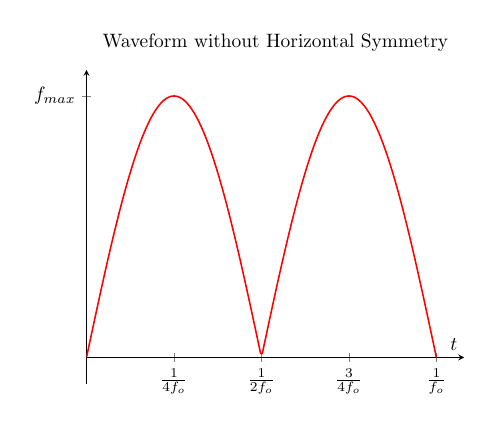
\begin{tikzpicture}[scale=0.7]
                \begin{axis}[
                    axis lines = middle,
                    xlabel = {$t$},
                    ylabel = {},
                    xmin = 0, xmax = 2*pi+0.5,
                    ymin = -0.1, ymax = 1.1,
                    samples = 200,
                    title = {Waveform without Horizontal Symmetry},
                    xtick = {pi/2, pi, 3*pi/2, 2*pi},
                    xticklabels = {$\frac{1}{4f_o}$, $\frac{1}{2f_o}$, $\frac{3}{4f_o}$, $\frac{1}{f_o}$},
                    ytick = {0, 1},
                    yticklabels = {0, $f_{max}$}
                ]
                
                \addplot [red, thick, domain=0:2*pi] {abs(sin(deg(x)))};
                
                \end{axis}
                
            \end{tikzpicture}
        \end{minipage}
        \hfill
        \begin{minipage}{0.49\textwidth}
            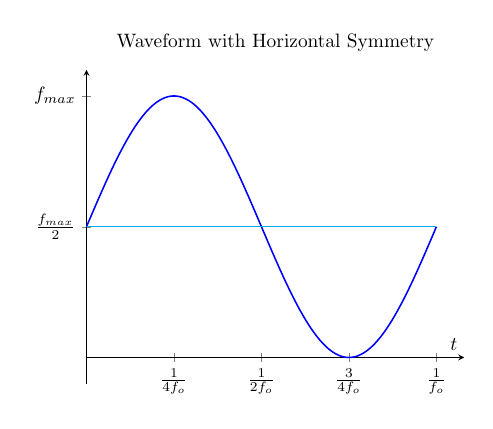
\begin{tikzpicture}[scale=0.7]
                \begin{axis}[
                    axis lines = middle,
                    xlabel = {$t$},
                    ylabel = {},
                    xmin = 0, xmax = 2*pi+0.5,
                    ymin = -0.1, ymax = 1.1,
                    samples = 200,
                    title = {Waveform with Horizontal Symmetry},
                    xtick = {pi/2, pi, 3*pi/2, 2*pi},
                    xticklabels = {$\frac{1}{4f_o}$, $\frac{1}{2f_o}$, $\frac{3}{4f_o}$, $\frac{1}{f_o}$},
                    ytick = {0, 0.5, 1},
                    yticklabels = {0, $\frac{f_{max}}{2}$, $f_{max}$}
                ]
                
                \addplot [blue, thick, domain=0:2*pi] {(sin(deg(x)) + 1)/2};
                \addplot [cyan, thick, domain=0:2*pi] {0.5};
                
                \end{axis}
                
            \end{tikzpicture}
        \end{minipage}
    }
    \vspace*{0.5cm} 

\end{center}

\noindent
The operation performed to the output is \(\texttt{out} = \frac{q}{2} + \frac{f_{max}}{2} = \frac{\texttt{q}}{2} + \texttt{HALF\_DATA} \).
When the horizontal symmetry is enabled the output must be inverted, so the output is \(\texttt{out} = -\frac{q}{2} + \frac{f_{max}}{2} = -\frac{\texttt{q}}{2} + \texttt{HALF\_DATA} \).

\vspace{1cm}
\begin{lstlisting}[language=Verilog, caption=Output calculation with horizontal mirroring, 
label=lst:DDFS_output_calculation ]
    //calculate the output
    reg [ADDR_WIDTH+1:0] act_cont;
    localparam HALF_DATA = 2**(DATA_WIDTH-1);
    always @(*) begin
    
        //not mirrored case
        q = HALF_DATA + (q_tmp >> 1) - 1;
        
        //select the correct counter for the wave we are using
        if(sin)
            act_cont = cont_rt;
        else 
            act_cont = cont;
        
        if(mirror_x && mirror_y) begin
            //third quarter or fourth quarter
            if( 
            ((act_cont > (2*MAX_LUT-1)) && (act_cont <= (3*MAX_LUT-1))) || 
            ((act_cont > (3*MAX_LUT-1)) && (act_cont <= (4*MAX_LUT-1))) 
            )
                q = HALF_DATA - (q_tmp >> 1) - 1;
                
        end else if(mirror_x) begin
            //second quarter or fourth quarter
            if(
            ((act_cont > (MAX_LUT-1)) && (act_cont <= (2*MAX_LUT-1))) || 
            ((act_cont > (3*MAX_LUT-1)) && (act_cont <= (4*MAX_LUT-1))) 
            )
                q = HALF_DATA - (q_tmp >> 1) - 1;
        
        end
            
    end
\end{lstlisting}
\vspace{1cm}

\noindent
The horizontal symmetry needs to be applied during the second and fourth quarters when vertical symmetry is not enabled. \\
When vertical symmetry is enabled, the period of the wave is \(2 \cdot T\), and horizontal symmetry must be applied in the third and fourth quarters. \\
To calculate the address, a global counter is used, and is performed the modulo operation with base \texttt{MAX\_LUT}.

\newpage
\noindent
The problem with this technique is that when the address moves from one quarter to another, if \texttt{f\_w} is greater than one, the address can start from a value bigger than zero. \\
For example, if \texttt{MAX\_LUT} is \(1024\) and \texttt{cont} is \(1000\), with \texttt{f\_w} equal to \(600\), the next value of \texttt{cont} is \(1000 + 600 = 1600\).\\
This means that \texttt{address} is equal to \texttt{cont} when it is \(1000\), but at the next clock cycle it becomes \(|1600|_{1024} = 576\).\\
Therefore, the \texttt{address} starts counting from \(0\), and in the next quarter of the wave it starts from \(576\).\\
This behavior causes the output waveform to be slightly different from period to period.\\
To avoid this, when the \texttt{address} is about to overflow, the \texttt{counter} is set to a multiple of \texttt{MAX\_LUT}, so that at the next cycle the \texttt{address} starts from \(|N \cdot 1024|_{1024} = 0\).

\vspace{1cm}
\begin{lstlisting}[language=Verilog, caption=Calculation of counter for DDFS address, 
label=lst:DDFS_cont_calculation ]
    if(cont < MAX_LUT-1) begin
        if(cont + (fw+1) >= MAX_LUT-1)
            cont <= MAX_LUT;
        else
            cont <= cont + (fw+1);
    end
    else if(cont < 2*MAX_LUT-1) begin
        if(cont + (fw+1) >= 2*MAX_LUT-1)
            cont <= 2*MAX_LUT;
        else
            cont <= cont + (fw+1);
    end
    else if(cont < 3*MAX_LUT-1) begin
        if(cont + (fw+1) >= 3*MAX_LUT-1)
            cont <= 3*MAX_LUT;
        else
            cont <= cont + (fw+1);
    end
    else if(cont < 4*MAX_LUT-1) begin
        if(cont + (fw+1) >= 4*MAX_LUT-1)
            cont <= 0;
        else
            cont <= cont + (fw+1);
    end
    else
        cont <= 0;
\end{lstlisting}
\vspace{1cm}

\paragraph{Sub-modules} \quad \\
Inside this module are instantiated two other modules

\begin{itemize}
    \item \textbf{Programmable frequency divider} to scale the clock frequency to lower values
    \item \textbf{Look Up Table} to store the digital samples for sinusoidal output
\end{itemize}

\newpage

\paragraph{Programmable frequency divider} \quad \\
We implemented a scalable frequency divider controlled by the \texttt{freq\_ctrl} \(3 bit\) signal to divide the output frequency with a coefficient ranging from \(2\) to \(1000000\).\\
This is useful to maintain a decent quality of the output wave, even with higher values of the frequency word.\\
With this method, using an input frequency of \(50MHz\), we can select the output frequencies of \(25MHz\), \(5MHz\), \(500kHz\), \(50kHz\), \(5kHz\), \(500Hz\), and \(50Hz\).\\
A \(20 bit\) counter is used, and the output is connected to the MSB of the counter.\\
The output clock is then generated with a \(0.5\) duty cycle by starting the counter when the MSB is 0 and, after half of the counter period, the MSB becomes 1; then the counter resets to the start.\\
When \texttt{freq\_ctrl} changes, the \texttt{start\_cnt} and \texttt{end\_cnt} registers are updated, and thus the counter restart condition also changes, avoiding conflicts.


\vspace{1cm}
\begin{lstlisting}[language=Verilog, caption=Programmable frequency divider,
    label=lst:Prog_freq_div ] 
    always @(posedge clk_in) begin
        if(rst_n == 1'b0) begin
            count <= start_cnt;
        end else if(count >= (end_cnt-1'b1))begin
            count <= start_cnt;
        end else begin
            count <= count + 1'b1; 	
        end
        
    end

    always @(*) begin
    
        case (freq_cntrl)
            
            0:begin 
                start_cnt = 20'h80000-1;
                end_cnt = start_cnt+2; 
            end
            1:begin
                start_cnt = 20'h80000-10/2;
                end_cnt = start_cnt + 10;
            end
            .
            .
            .
            
            6:begin
                start_cnt = 20'h80000-1000000/2;
                end_cnt = start_cnt + 1000000;
            end
            default:begin
                start_cnt = 20'h80000-1000000/2;
                end_cnt = start_cnt + 1000000;
            end
            
        endcase 
    
        clk_out = count[19];
        
    end
    
\end{lstlisting}
\vspace{1cm}

\newpage

\paragraph{Look Up Table} \quad \\
The LUT is a pre-initialized ROM instantiated inside the FPGA with the samples of a quarter of a sinusoidal wave. \\
The samples stored in the ROM are \(12 bit\) samples calculated as follows 

\vspace{0.5cm}
\[
    \texttt{sample}[n]_{12 bit} = sin\left(\frac{n}{\texttt{LUT\_DIM} - 1} \cdot \frac{\pi}{2}\right)_{12 bit}
\]
\vspace{0.5cm}

\noindent
The \texttt{LUT\_DIM} is choose to be \(2^{10}\), so the LUT is a \((12 \text{x} 1024) bit\) ROM inside the FPGA.

\newpage
\subsubsection{Keypad frequency select module}

This module reads the button pressed on the keypad every \(N\) clock cycles. \\
The keypad is used to enter the frequency of the wave, and the output of this module is the frequency in BCD or \textbf{binary-coded decimal} representation. \\
Inside the module, there is a converter network that converts the frequency value into a combination of \texttt{f\_w} and \texttt{freq\_cntrl}, which are the inputs of the DDFS module used to control the output wave frequency.

\vspace{0.5cm}
\begin{figure}[h!]
    \centering
    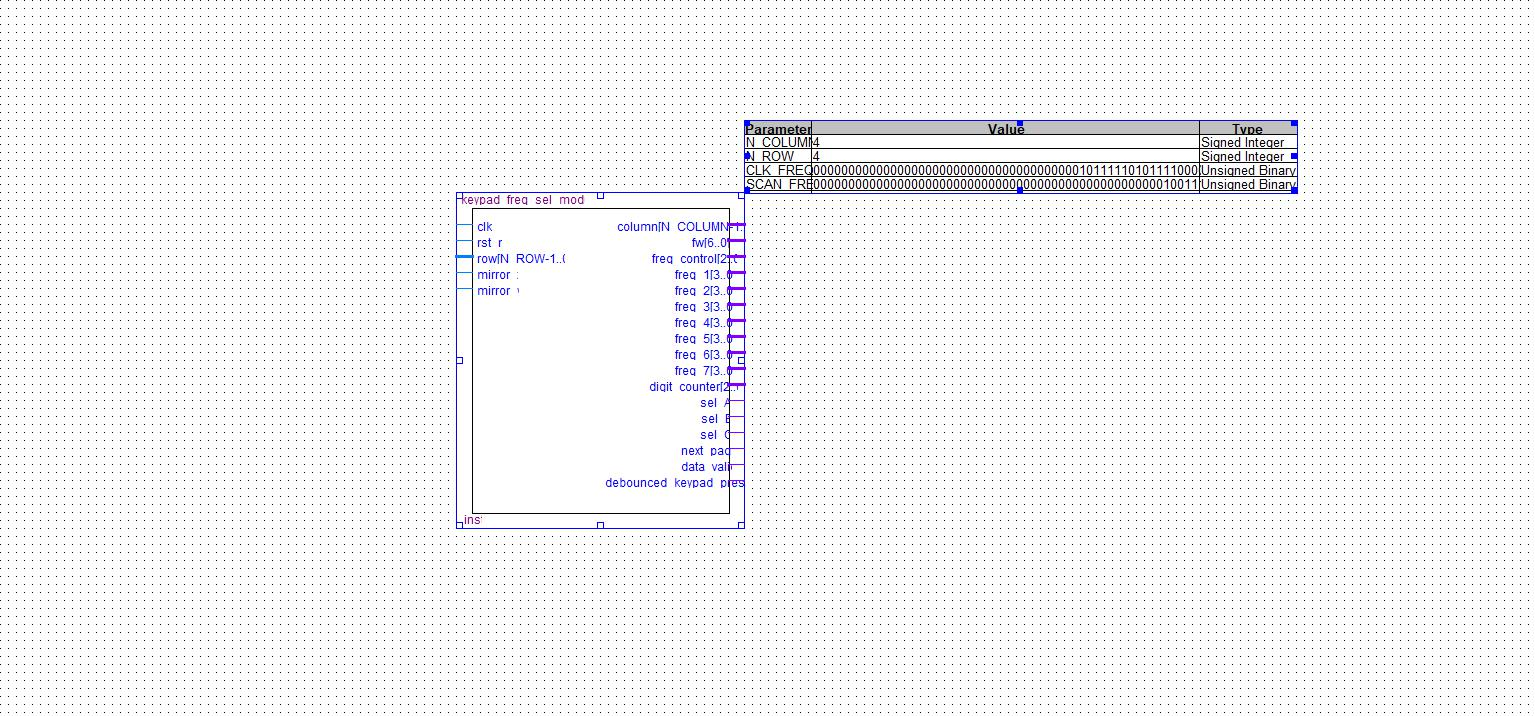
\includegraphics[width=0.8\textwidth, trim={8cm 3cm 3cm 1.5cm}, clip]{img/keypad_freq_sel.jpg}
    \caption{Keypad frequency select module}
    \label{fig:keypad_module}
\end{figure}
\vspace{0.5cm}

\paragraph{I/O interface} \quad \\
The ports used to connect this module to other modules or to the external pins of the FPGA are the following:

\begin{itemize}

    \item \texttt{clk, rst\_n} \\
    are the clock and the synchronous reset pins.

    \item \texttt{row} \\
    this is the input pin from the keyboard. \\
    This pins need to be connected to the internal pullup of the FPGA, because the keypad matrix, when a button is not pressed, leave the line floating. \\
    Every bit of this word is connected to a row line of the keypad.

    \item \texttt{mirror\_x, mirror\_y} \\
    these are the mirroring pins of the output wave; if the output wave is mirrored, the LUT must be read two or four times (depending on how many mirroring effects are applied to the wave) every period. \\
    This means that the \texttt{f\_w} and \texttt{freq\_control} values depend on the value of \texttt{mirror\_x} and \texttt{mirror\_y}.
    

    \item \texttt{column} \\
    this output pin is connected to the keypad, and is used to enable the column before reading a row. \\
    By enabling a column and reading the row values is possible to determine which button is pressed.

    \item \texttt{f\_w, freq\_control} \\
    this outputs goes to the DDFS module to set the frequency of the output wave.

    \item \texttt{freq\_1, freq\_2, ... ,freq\_7} \\
    this is the 7 digits of the output frequency expressed in BCD representation.

    \item \texttt{digit\_counter} \\
    this output represent the number of the frequency digits.

    \item \texttt{sel\_A, sel\_B} \\
    these outputs are toggled every time the A and B buttons of the keypad are pressed. \\
    This can be useful because the VGA DAC has three \(10 bit\) inputs, so it is possible to instantiate two DDFS modules connected to each DAC input, and these pins can individually enable each DDFS module.

    \item \texttt{next\_page, prev\_page} \\
    this output is connected to LCD module to change the wave to be visualized.

    \item \texttt{data\_valid, debounced\_keypad\_pressed} \\
    are test outputs used for debugging.
    
\end{itemize}

\paragraph{Parameters} \quad \\
The parameters of this module are:

\begin{itemize}

    \item \texttt{N\_COLUMN, N\_ROW} \\
    are the number of rows and column of the keypad module used

    \item \texttt{SCAN\_FREQ} \\
    this is the frequency used to perform the keypad scanning. \\
    If the scan operation is performed too rapidly, the parasitic capacitance of the buttons, in series with the pull-up resistors, can create reading problems. \\
    The scan frequency value used is \(10kHz\).

    \item \texttt{CLK\_FREQ} \\
    is the clock frequency of the clock connected to this module. \\
    Is used to synchronize the timers for the debounce circuit and the scanning frequency of the keypad.
    
\end{itemize}

\paragraph{Verilog code} \quad \\
The module is made of a single sequential network that checks every clock cycle whether the \texttt{data\_valid} signal (from the sub-module that reads the keypad buttons) is high, and reads which button is pressed in that case. \\
The first problem is that the button bounces significantly before stabilizing in one position. \\
For this reason, a debounce circuit has been implemented, with a timer that waits for approximately \(100ms\) after the button is pressed before considering the button as pressed.

\vspace{0.5cm}
\begin{lstlisting}[language=Verilog, caption=Debounce circuit, 
label=lst:debounce_circuit ]
    always @(posedge clk) begin
        if(rst_n == 0) begin
            //reset condition
            debounce_cont <= 0;
            debounced_keypad_pressed <= 1'b0;
        end else if(clk_ena == 1) begin
            if(out_keys == 16'd0) begin
                debounce_cont <= 0;
                debounced_keypad_pressed <= 1'b0;
                out_keys_sync <= out_keys_sync;
            end else begin
                debounce_cont <= debounce_cont + 1;
                if(debounce_cont >= DEBOUNCE_CYCLE) begin
                    debounce_cont <= DEBOUNCE_CYCLE;
                    debounced_keypad_pressed <= 1'b1;
                    out_keys_sync <= out_keys;
                end
            end
        end else begin
            debounce_cont <= debounce_cont;
            debounced_keypad_pressed <= debounced_keypad_pressed;
            out_keys_sync <= out_keys_sync;
        end
    end
\end{lstlisting}
\vspace{0.5cm}

\newpage
\noindent
The second problem is that a button is usually pressed for too long; for this reason, a flag has been instantiated to check if the button has been released. \\
This flag makes it possible to perform an action only once, even if the button remains pressed for many clock cycles.

\vspace{0.5cm}
\begin{lstlisting}[language=Verilog, caption=Flag to avoid multiple operation with a single press, 
label=lst:pressed_button_flag ]
    if(data_valid == 1) begin   
        if(debounced_keypad_pressed == 0) begin
            //flag reset
            button_pressed <= 1'b0;
        end
        if(debounced_keypad_pressed == 1 && button_pressed == 0) begin
    
            .
            .
            .
            
            //flag set
            button_pressed <= 1'b1;
        end
    end
\end{lstlisting}
\vspace{1cm}

\noindent
Now we have to define the behavior of the machine upon the press of each button. \\
When multiple buttons are pressed simultaneously, the machine does nothing by default. \\
When a number is pressed, the machine shifts the digits of the frequency number to the left and writes the pressed number in the place of the least significant digit. \\
If a new number have to be selected, the flag \texttt{number\_not\_sel} is high and the number become the digit pressed.

\vspace{0.5cm}
\begin{lstlisting}[language=Verilog, caption=Number digit pressed on the keypad, 
label=lst:number_key_pressed ]
    // ---- NUMBER KEY PRESSED ---- //
    
    (16'd1 << 0): begin
        if(number_not_sel == 1) begin
            {freq_7, freq_6, freq_5, freq_4, freq_3, freq_2, freq_1} <= 1;
            digit_counter <= 3'd1;
            number_not_sel <= 1'b0;
        end else if(digit_counter < 7) begin
            //shift right and write the first digit
            {freq_7, freq_6, freq_5, freq_4, freq_3, freq_2, freq_1} <=
            {freq_6, freq_5, freq_4, freq_3, freq_2, freq_1, 4'd1};
            //increase the number of digit
            digit_counter <= digit_counter + 1;
        end
    end
    
    .
    .
    .
    
    // ---- DEFAULT CONDITION ---- //
                
    default: begin
        {freq_7, freq_6, freq_5, freq_4, freq_3, freq_2, freq_1} <=
        {freq_7, freq_6, freq_5, freq_4, freq_3, freq_2, freq_1};
        digit_counter <= digit_counter;
    end 
\end{lstlisting}
\vspace{0.5cm}

\newpage
\noindent
The letter buttons toggle the \texttt{sel\_A} and \texttt{sel\_B} outputs, the C and D buttons of the keypad are used to send the next page or previous page signals to the LCD module. \\
The last two buttons of the keypad are used to confirm the frequency value written
or to erase the digits.

\vspace{0.5cm}
\begin{lstlisting}[language=Verilog, caption=Confirm or erase button pressed on the keypad, 
label=lst:confirm_erase_key_pressed ]
    // ---- CONFIRM OR ERASE KEY PRESSED ---- //
                    
    (16'd1 << 14): begin
        if(digit_counter > 0) begin
            //digit erased, shift left the digit
            {freq_7, freq_6, freq_5, freq_4, freq_3, freq_2, freq_1} <=
            {4'd0, freq_7, freq_6, freq_5, freq_4, freq_3, freq_2};							
            //decrease the number of digit
            digit_counter <= digit_counter - 1;
        end
        else begin
            {freq_7, freq_6, freq_5, freq_4, freq_3, freq_2, freq_1} <=
            {BCD_7, BCD_6, BCD_5, BCD_4, BCD_3, BCD_2, BCD_1};
            //store the previous number of digit
            digit_counter <= digit_counter_BCD;
            number_not_sel <= 1'b1;
        end
    end 
    
    (16'd1 << 12): begin
        //frequency confirmed, save the frequency value
        {BCD_7, BCD_6, BCD_5, BCD_4, BCD_3, BCD_2, BCD_1} <= 
        {freq_7, freq_6, freq_5, freq_4, freq_3, freq_2, freq_1};
        //load the actual number of digit
        digit_counter_BCD <= digit_counter;
        number_not_sel <= 1'b1;
    end 
\end{lstlisting}
\vspace{0.5cm}

\noindent
When a value is confirmed, the flag \texttt{number\_not\_sel} is set to one, so when a digit is pressed, the new number starts to be written from the least significant digit. \\
When a digit is erased, the number is shifted to the right and the most significant digit become a zero.

\newpage

\paragraph{Sub-modules} \quad \\
Inside this module are instantiated three other modules

\begin{itemize}
    \item \textbf{Keypad reader module} to read the button values of the keypad.
    \item \textbf{BCD to C1 converter} to convert the frequency value from BCD to C1 representation.
    \item \textbf{DDFS frequency converter} to convert the C1 frequency value into a combination of \texttt{f\_w} and \\
    \texttt{freq\_control} used to control the DDFS module.
\end{itemize}

\paragraph{Keypad reader module} \quad \\
This module uses a shift register connected to the column lines to enable a different column every clock cycle. \\
The logic is reversed: a column is considered enabled when it is pulled low, and a row is considered active when the line value is low. \\
This choice was made because the FPGA GPIOs can be defined with internal \(25 k\Omega\) pull-up resistors but no internal pull-downs. \\
After \(N_{col}\) clock cycles, where \(N_{col}\) is the number of columns of the keypad, the controller pulls up the \texttt{data\_valid} pin to indicate that the output of the module contains the pressed button. \\
Every clock cycle, a counter called \texttt{i\_column} increases, and when the value of the counter reaches \(N_{col}\), it activates \texttt{data\_valid}. \\
At each clock cycle, a different column is enabled, and the value of the pressed row is stored in an output vector called \texttt{out\_keys}. \\
The structure of the output value is a \texttt{bidimensional-vector}, that has been implemented using a technique called \textbf{array flattening}. \\
The array flattening technique consists of dividing the array into consecutive sub-arrays representing the rows of the matrix, where the columns correspond to the values inside the sub-arrays. \\
The flattened array contains \(N_{col} \cdot N_{row}\) elements, and the index of each element is calculated from the \(i_{col}\) and \(i_{row}\) indices using the following formula \( i = N_{row} \cdot i_{col} + i_{row}\).

\vspace{0.5cm}
\begin{figure}[h!]
    \centering
    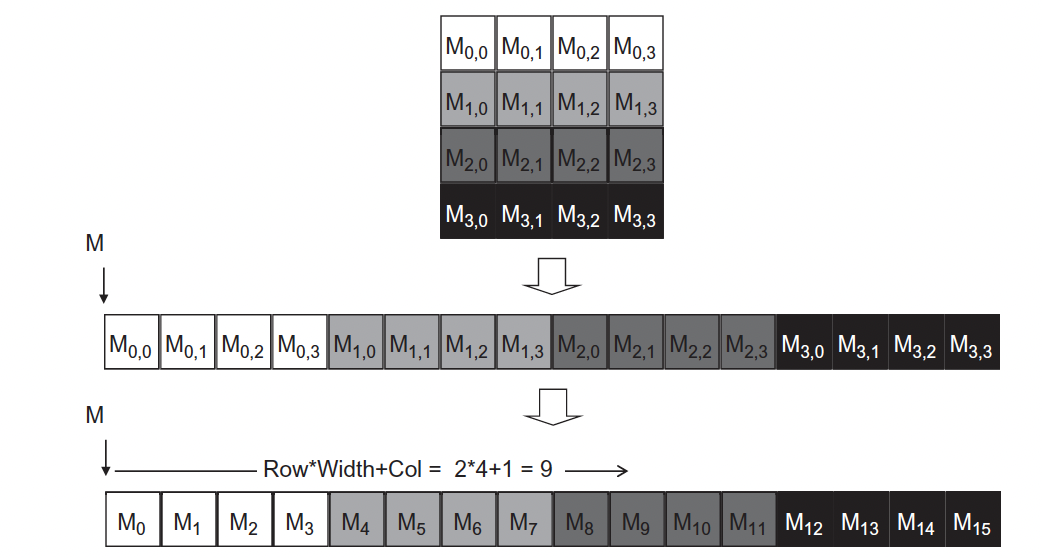
\includegraphics[width=0.8\textwidth, clip]{img/array flattening.png}
    \caption{Array flattening technique}
    \label{fig:arr_flat}
\end{figure}
\vspace{0.5cm}

\newpage
\noindent
The shift register connected to the columns is implemented with a combinatorial network that reads the value of \texttt{i\_column} and pulls down the corresponding line. \\
To prevent the module from sampling the row values too close to the change of column enable, the \texttt{i\_column} values range from \(0\) to \(2 \cdot \texttt{N\_COLUMN}\). \\
When \texttt{i\_column} is odd, the column is enabled; when it is even, the row is read. \\
By doing this, the reading operation occurs one clock cycle after the column enabling operation.


\vspace{0.5cm}
\begin{lstlisting}[language=Verilog, caption=Shift register implementation ]
    //assign the output values at the column of the keypad
    integer i;
    always @(*) begin
        //default values
        i = 0;
        column = ~0;
        
        //check if i_column is in range
        if(i_column <= 2*N_COLUMN) begin
            for(i=0; i<N_COLUMN; i=i+1) begin
                if(i == (i_column >> 1)) begin
                    column[i] = 0;
                end else begin
                    column[i] = 1;
                end
            end
        end
        
    end
\end{lstlisting}
\vspace{0.5cm}

\noindent
Another combinatorial network updates a flattened vector that contains the button pressed for the currently enabled column.

\vspace{0.5cm}
\begin{lstlisting}[language=Verilog, caption=Button reading implementation]
    //read the button values from the keypad
    integer i_col, i_row;
    always @(*) begin
        //default values
        i_col = 0;
        i_row = 0;
        
        //read button cycles
        for(i_col=0; i_col<N_COLUMN; i_col=i_col+1) begin
            for(i_row=0; i_row<N_ROW; i_row=i_row+1) begin
                if(row[i_row] == 0 && i_col == (i_column >> 1)) begin
                    key_pressed[i_col*N_ROW + i_row] = 1; 
                end else begin
                    key_pressed[i_col*N_ROW + i_row] = 0; 
                end
            end
        end
        
    end
\end{lstlisting}
\vspace{0.5cm}

\noindent
Every two clock cycle, the output vector is updated with the button pressed for each column and after \(2 \cdot N_{col}\) cycles the reading cycle is done and data output is valid.

\newpage
\noindent
The two main issues encountered when reading the keypad are:
\begin{itemize}
    \item The button press event is asynchronous.
    \item The scan frequency cannot be too high due to the parasitic capacitance of the buttons and the pull-up resistors.
\end{itemize}

\noindent
For the first issue, the module provides a flip-flop chain directly connected to the keypad inputs, reducing the probability of metastability problems.

\vspace{0.5cm}
\begin{lstlisting}[language=Verilog, caption=flip-flop chain to reduce metastability problem occur]
    //latch chain to reduce metastability problems
    reg [N_ROW-1:0] row_1, row_2, row_sync;
    always @(posedge clk) begin
        if(rst_n == 0) begin
            //reset condition
            row_1 <= 0;
            row_2 <= 0;
            row_sync <= 0;
        end
        else begin
            row_sync <= row_2;
            row_2 <= row_1;
            row_1 <= row;
        end
    end
\end{lstlisting}
\begin{center}
    \vspace{0.5cm}
    \scalebox{0.7}{
        \begin{tikzpicture}
        	% Paths, nodes and wires:
        	\node[flipflop D, fill=cyan!30!white] at (3.12, 5.16){};
        	\node[flipflop D, fill=cyan!30!white] at (7.13, 5.16){};
        	\node[flipflop D, fill=cyan!30!white] at (11.13, 5.16){};
        	\draw (4.25, 6) -- (6, 6);
        	\draw (8.25, 6) -- (10, 6);
        	\draw (2, 6) |- (1, 6);
        	\draw (6.01, 4.32) -| (5.25, 3);
        	\draw (10.01, 4.32) -| (9.25, 3);
        	\draw (9.25, 3) -- (1, 3);
        	\draw (2, 4.32) -| (1.25, 3);
        	\draw (1, 3) -- (0.25, 3);
        	\draw (1, 6) -- (0.25, 6);
        	\node[circ] at (5.25, 3){};
        	\node[circ] at (1.25, 3){};
        	\node[shape=rectangle, minimum width=0.715cm, minimum height=0.465cm] at (0.625, 6.25){} node[anchor=north west, align=left, text width=0.327cm, inner sep=6pt] at (0.25, 6.5){in};
        	\node[shape=rectangle, minimum width=0.84cm, minimum height=0.465cm] at (0.563, 3.25){} node[anchor=north west, align=left, text width=0.452cm, inner sep=6pt] at (0.125, 3.5){clk};
        	\draw (13.25, 6) |- (12.25, 6);
        	\node[shape=rectangle, minimum width=0.965cm, minimum height=0.465cm] at (13, 6.25){} node[anchor=north west, align=left, text width=0.577cm, inner sep=6pt] at (12.5, 6.5){out};
        \end{tikzpicture}
    }
    \vspace{0.5cm}
\end{center}

\noindent
To solve the second issue, the module includes a clock enable signal generated by an internal counter. Each time the clock enable signal is asserted, the synchronized operations are performed. \\
The clock enable signal is also forwarded to the keypad frequency selection module.

\vspace{0.5cm}
\begin{lstlisting}[language=Verilog, caption=Clock enable signal generation]
    //clock enable generator
    localparam FREQ_DIV = (CLK_FREQ/SCAN_FREQ>3) ? CLK_FREQ/SCAN_FREQ : 3;
    integer clock_div_cont;
    always @(posedge clk) begin
        if(rst_n == 0) begin
            //reset condition
            clock_div_cont <= 0;
            clk_ena <= 1'b0;
        end
        else begin
            clock_div_cont <= clock_div_cont + 1;
            clk_ena <= 1'b0;
            if (clock_div_cont >= FREQ_DIV) begin
                clock_div_cont <= 0;
                clk_ena <= 1'b1;
            end
        end
    end
\end{lstlisting}
\vspace{0.5cm}

\noindent
The flip-flop chain introduces a delay, as the output data is delayed with respect to the input data by three clock cycles.\\
For this reason, the \texttt{FREQ\_DIV} parameter is defined to be greater than three, ensuring that the output delay introduced by the chain is absorbed before the next reading operation.

\paragraph{BCD to C1 converter} \quad \\
This module takes as input the value to be converted from BCD representation and converts it into a C1 representation value. \\
To perform this operation, the value must be calculated as follows

\[
    n_{C1} = \sum_{i=0}^{\texttt{n\_digit}} a_i \cdot 10^i
\]

\noindent
This operation instantiates many multipliers, which are hardware-expensive; for this reason, every power of \(10\) is decomposed into a sum of powers of two

\[
    n_{C1} = \sum_{i=0}^{\texttt{n\_digit}} a_i \cdot 10^i
           = \sum_{i=0}^{\texttt{n\_digit}}
             \left[ a_i \cdot \left( \sum_{j} b_j \cdot 2^j \right) \right] \qquad b_j \in \{1,0\}
\]

\noindent
Doing this transforms every multiplication into a combination of additions and left shifts, which are less expensive in terms of hardware primitives instantiated on the FPGA.

\paragraph{DDFS frequency converter} \quad \\
This module reads the frequency value to be sent to the DDFS module and converts it into a combination of \texttt{f\_w} and \texttt{freq\_control}, which are the frequency-control inputs of the DDFS module. \\
The output frequency of the DDFS module is calculated as follows

\[
    f_{out} = \frac{f_{clk}}{N} \cdot \frac{f_w + 1}{\texttt{LUT\_DIM}}
    \qquad 
    f_w \in [0, 127]
\]

\noindent
where \(\frac{f_{clk}}{N}\) is the divided clock frequency from the frequency divider, and \(f_w\) is the frequency word.
The output frequency range for each divided frequency is (in our case \(\texttt{LUT\_DIM} = 2^{10} = 1024\))

\[
    f_{out} \in [ \frac{f_{clk}}{N \cdot \texttt{LUT\_DIM}}, \frac{f_{clk} \cdot 128}{N \cdot \texttt{LUT\_DIM}} ] \xrightarrow{\texttt{LUT\_DIM} = 1024}
    [ \frac{f_{clk}}{N \cdot 1024}, \frac{f_{clk}}{N \cdot 8} ]
\]

\noindent
For any selected output frequency, the module chooses a value of \(N\) such that the desired frequency lies within the range
\([ \frac{f_{clk}}{N \cdot 1024},\ \frac{f_{clk}}{N \cdot 8} ]\). \\
Once the value of \(N\) has been chosen, to calculate \(f_w\) the formula is the following

\[
    f_w = f_{out} \cdot \frac{N \cdot \texttt{LUT\_DIM}}{f_{clk}} = f_{out} \cdot \frac{N \cdot 2^{10}}{f_{clk}}
\]

\noindent
The problem with this formula is that, even if the value of \(f_{clk}/N\) is pre-calculated, the synthesizer instantiate a divider to do the \(f_{out} / f_{clk} \) operation, and this have to be done for every frequency range, so the divider instantiated are more than one. \\
Instantiating a divider is challenging because it results in a large combinational network and, unless the operation is pipelined, it significantly reduces the maximum operating frequency of the design. \\
Another drawback of instantiating a divider is that it occupies a considerable amount of device resources. \\
An alternative approach is to use the following formula

\[
    f_w = \frac{2^{64}}{f_{clk}} \cdot \frac{f_{out} \cdot N}{2^{54}} = K \cdot \frac{f_{out} \cdot N}{2^{54}}
\]

\noindent
using this method, \(K\) can be pre-calculated, and the division for \(2^{54}\) can be done with a shift left operation. \\
In this way, the compiler can replace the division with internal multipliers, thus avoiding the instantiation of hardware dividers. \\
Multipliers are also large combinatorial networks, but they are smaller and faster compared to dividers.

\newpage

\subsection{LCD module}
In this section we have a description of the driving mechanism used for the LCD module. \\
The goal is to display a character sequence relative to the selected wave function name and its frequency, and to change each output wave (and its displayed name) using two buttons to move to the previous or next wave function. \\
To store the character to display a LUT is used, containing, for each entry, a 9 bit code addressable with a page address and a character address as we will see later on. 

\vspace{0.5cm}
\begin{figure}[h!]
    \centering
    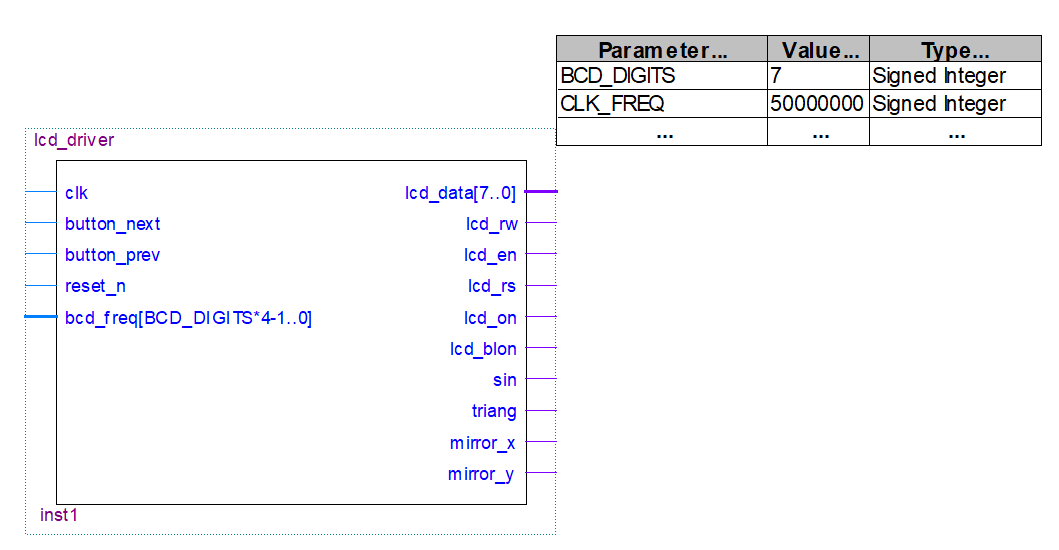
\includegraphics[width=0.8\textwidth]{img/LCD_module_.png}
    \caption{LCD driver module}
    \label{fig:LCD_module}
\end{figure}
\vspace{0.5cm}

\paragraph{I/O interface} \quad \\
The ports used to connect this module to other modules or to the external pins of the FPGA are the following:

\begin{itemize}

    \item \texttt{clk, reset\_n} \\
    are the clock and the synchronous reset pins

    \item \texttt{button\_next, button\_prev} \\
    these are connected to the input buttons used for cycling through each page and so each wave function to display 

    \item \texttt{bcd\_freq} \\
    this input is received from the "Keypad frequency select module" and it is the BCD converted frequency to display on the screen. Each decimal digit to display needs 4 bit to be represented in BCD, so the parameter \texttt{BCD\_DIGITS} is used to instantiate the correct bit value for the digits we want to display

    \item \texttt{lcd\_data} \\
    this is the 8 bit data bus connected to the LCD controller used to write instructions in the IR (instruction register) or the 8 bit ASCII code the DR (data register)

    \item \texttt{lcd\_en} \\
    this pin enable the writing cycle from the data bus to the internal registers of the LCD controller (IR or DR)

    \item \texttt{lcd\_rs} \\
    this pin is used to select the writing on the IR or DR (register select) 

    \item \texttt{lcd\_on} \\
    this pin control the power supply of the LCD and it is always high 

    \item \texttt{lcd\_blon} \\
    this pin control the backlight of the LCD and it is always on 

    \item \texttt{sin ,triang} \\
    these pins are sent to the DDFS module to enable the output of the selected wave function 

    \item \texttt{mirror\_x ,mirror\_y} \\
    these pins are sent to the DDFS module to change the mirroring options of the waveform 
    
\end{itemize}

\paragraph{Parameters} \quad \\
The parameters of this module are:

\begin{itemize}

    \item \texttt{BCD\_DIGITS} \\
    are the number of frequency digit to display on the module.

    \item \texttt{CLK\_FREQ} \\
    is the clock frequency of the clock connected to this module. \\
    Is used to synchronize the timers for the debounce circuits and to respect the timing constrain for the communication with the LCD.
    
\end{itemize}

\paragraph{Verilog code} \quad \\
The LCD module is composed of 2 Synchronous Finite State Machines. One operates to display the name of the selected function in the first row of the screen, while the other continuously displays the selected frequency in the second row of the display when the other FSM is waiting for a button pressure (and release) to change page. \\
To implement two different FSM in the same Verilog code we need to multiplex the shared registers between the two FSM, in our case the registers to be multiplexed are the ones responsible for the LCD driving: \texttt{lcd\_rs}, \texttt{lcd\_data}, \texttt{lcd\_en}. \\
At the end of this combinational always block is present the extrapolation of each BCD number \\ 
(\texttt{bcd\_number}) from the input bit vector (\texttt{bcd\_freq}), using a reverse indexing strategy. 

\vspace{1cm}
\begin{lstlisting}[language=Verilog, caption=Registers multiplexing for FSMs ]
    always @(*) begin
        if( state != WAIT_BUTTON_SHORT && state != WAIT_BUTTON_RELEASE ) begin
            lcd_rs_reg = lut_out[DATA_WIDTH-1];
            lcd_data_reg = lut_out[DATA_WIDTH-2:0];
            lcd_en_reg = lcd_en_cntr;
        end else begin 
            lcd_rs_reg = lcd_rs_freq;
            lcd_data_reg = lcd_data_freq; 		 
            lcd_en_reg = lcd_en_freq;
        end
        //Each BCD (binary coded decimal) digit needs 4 bits
        //number extracted from most significant BCD 
        //to least significant BCD (reverse index)
        bcd_number = bcd_freq[(LAST_BCD_INDEX-(n_index*4))+:BCD_BITS]; 
        if( bcd_number >= 4'd9 ) begin
            bcd_number = 9;
        end
    end
\end{lstlisting}
\vspace{1cm}

\newpage
\noindent
The core of the process to send data to the LCD is here, this mechanism is present in both FSMs, even if in the following piece of code we are going to analyze the first FSM. \\
At the start of the system it is necessary to wait more than 15ms as stated on the datasheet of the \\ \texttt{CFAH1602B-TMC-JP}.
Each new instruction or character writing starts in the \texttt{SETUP} state, the chip enable is set low and a wait time is scheduled, then in the \texttt{WRITE\_DATA} state the enable is set high enabling the sampling of the data to send to the LCD controller, after that the enable is set low again, and a wait for the execution (in the \texttt{WAIT\_EXEC}) is needed before going to the next state, the one responsible to select the next character (or instruction) and eventually the page. 

\noindent
\vspace{1cm}
\begin{lstlisting}[language=Verilog, caption=Sending data to LCD ]
    case (state)
    
        // Wait for more than 15ms at power on 
        POWER_ON: begin
            lcd_en_cntr <= 0;
            counter <= counter + 1'b1;
            if (counter >= wait20ms) begin
                state <= SETUP ;
                counter <= 0;
            end				 
        end
        
        // Setup time wait 
        SETUP: begin
            lcd_en_cntr <= 0;
            counter <= counter + 1'b1;
            if (counter >= wait40us) begin 
                state <= WRITE_DATA;
                counter <= 0;
            end
        end

        // Enable pulse high 
        WRITE_DATA: begin
            lcd_en_cntr <= 1;
            counter <= counter + 1'b1;
            if (counter >= wait1ms) begin 
                state <= WAIT_EXEC; 
                counter <= 0;
            end
        end

        // Wait instruction execution 
        WAIT_EXEC: begin
            lcd_en_cntr <= 0;
            counter <= counter + 1'b1;
            if (counter >= wait2ms) begin 
                char_index <= char_index + 1'b1;	
                state <= PAGE_SELECT; 
                counter <= 0;
            end
        end

        PAGE_SELECT: begin

        .
        .
        .
        
    endcase
\end{lstlisting}
\vspace{1cm}

\newpage

\paragraph{Text LUT instance} \quad \\
A LUT is instantiated with the instructions and ASCII coded characters needed to display the first row of the screen, the one related to the name of the selected waveform and the first two opening pages. \\
This particular LUT is addressable with 2 indexes, one that divides the LUT in pages (\texttt{page\_index}), for a maximum of 32 pages. \\
Each page is composed of 64 memory locations, addressable with the index \texttt{char\_index}. \\
Each address outputs a 9 bit value which has its MSB related to the register select signal (\texttt{lcd\_rs}) to send to the LCD controller, and the remaining 8 bits are related to the data bus (\texttt{lcd\_data}). The resulting dimension of the LUT is:     
\[
    \texttt{TEXT\_LUT\_DIM} = 32\cdot 64\cdot 9 = 2^{11}\cdot 9 = 18432 \texttt{bits} \simeq 18 \texttt{Kb}
\]

\vspace{1cm}
\begin{lstlisting}[language=Verilog, caption=LUT instance ]
    // text LUT instance
    localparam DATA_WIDTH = 9;
    localparam ADDR_WIDTH = 6;
    localparam PAGE_ADDR_WIDTH = 5;
    reg [ADDR_WIDTH-1:0] char_index = 0;
    reg [PAGE_ADDR_WIDTH-1:0] page_index = 0;
    wire [DATA_WIDTH-1:0] lut_out;  
    text_lut #(
        .DATA_WIDTH(DATA_WIDTH),
        .ADDR_WIDTH(ADDR_WIDTH),
        .PAGE_ADDR_WIDTH(PAGE_ADDR_WIDTH)
    ) text_lut_inst (
        .addr(char_index),
        .page(page_index),
        .clk(clk),
        .q(lut_out) 
    );
\end{lstlisting}
\vspace{1cm}

\newpage

\paragraph{First FSM: displaying wave function name} \quad \\
In the \texttt{PAGE\_SELECT} state a sub state strategy is used for each page. \\
The LUT is scanned from the first entry of each page by progressively incrementing \texttt{char\_index} (in the \texttt{WAIT\_EXEC} state), repeating the states cycle \texttt{SETUP}, \texttt{WRITE\_DATA}, \texttt{WAIT\_EXEC}. \\
At each new address, the output of the LUT drives the \texttt{lcd\_rs\_reg} and \texttt{lcd\_data\_reg}. \\
This cycle continues until an @ (hat sign) coded in ASCII is detected, or in case of an error, the end of the page is reached, and an exclusive page signaling the error is displayed. \\
While the first two pages are only used to display information about the project, thus they are displayed for only 2 seconds and automatically shifted, the page starting with the wave function selection capability needs to implement a button press detection and release before displaying a new page.  

\vspace{1cm}
\begin{lstlisting}[language=Verilog, caption= Page selection Sub State Machine ]
    PAGE_SELECT: begin
				
        case(sub_state)

            // DDFS Tonarini Aliberti
            PAGE0: begin
                if (char_index < (2**ADDR_WIDTH)-1) begin
                    if (lcd_data_reg == 8'h40) begin
                        char_index <= 0;
                        page_index <= PAGE1;
                        sub_state <= PAGE1;	
                        state <= WAIT;	
                    end else begin
                        state <= SETUP;
                    end
                end else begin 
                    char_index <= 0; 
                    sub_state <= PAGE_ERROR; 
                end
            end
            
            // Select wave function 
            PAGE1: begin
                if (char_index < 2**ADDR_WIDTH-1) begin
                    if (lcd_data_reg == 8'h40) begin
                        char_index <= 0;
                        page_index <= PAGE2;
                        sub_state <= PAGE2;
                        state <= WAIT;	
                    end else begin
                        state <= SETUP ;
                    end
                end else begin 
                    char_index <= 0; 
                    sub_state <= PAGE_ERROR; 
                end 
            end
            
            .
            .
            .
                
        endcase

    end
\end{lstlisting}
\vspace{1cm}

\newpage
\noindent   
The following code shows the states of the first FSM used to wait for a button to be pressed and released when selecting the wave function. \\
A de-bounce technique is implemented with a 10ms sensing time, and the \texttt{page\_index} is incremented or decremented based on which of the buttons is pressed. 

\vspace{1cm}
\begin{lstlisting}[language=Verilog, caption= Button press and release ]
    WAIT: begin
        counter <= counter + 1'b1;
        if (counter >= wait2s) begin 
            state <= SETUP; 
            counter <= 0;
        end
     
    end

    WAIT_BUTTON_SHORT: begin 			     
        if(button_next == 1'b0 || button_prev == 1'b0) begin 
            btn_counter <= btn_counter + 1'b1;
            if (btn_counter >= wait10ms) begin
                state <= WAIT_BUTTON_RELEASE ;
                btn_counter <= 0;
                    if (button_next == 1'b0) begin
                        btn_pressed <= BTN_NEXT;
                    end else begin
                        btn_pressed <= BTN_PREV;
                    end
            end			
        end else begin
            btn_counter <= 0;
            state <= WAIT_BUTTON_SHORT;
        end					
    end		 
         
    WAIT_BUTTON_RELEASE: begin 			     
        if(button_next == 1'b1 && btn_pressed == BTN_NEXT) begin 
            btn_counter <= btn_counter + 1'b1;
            if (btn_counter >= wait10ms) begin 
                state <= SETUP;
                btn_counter <= 0;								
                if (page_index >= PAGE_FIRST && page_index < PAGE_LAST) begin
                    page_index <= page_index + 1'b1;
                end else if ( page_index == PAGE_LAST ) begin
                    page_index <= PAGE_FIRST;
                end							
            end		
        end else if (button_prev == 1'b1 && btn_pressed == BTN_PREV) begin
            btn_counter <= btn_counter + 1'b1;
            if (btn_counter >= wait10ms) begin 
                state <= SETUP;
                btn_counter <= 0;								
                if (page_index > PAGE_FIRST && page_index <= PAGE_LAST) begin
                    page_index <= page_index - 1'b1;
                end else if ( page_index == PAGE_FIRST ) begin
                    page_index <= PAGE_LAST;
                end							
            end
        end else begin
            state <= WAIT_BUTTON_RELEASE;
            btn_counter <= 0;
        end				
    end
\end{lstlisting}
\vspace{1cm}

\paragraph{Second FSM: displaying wave function frequency} \quad \\
This FSM is used to show the frequency of the selected wave function on the second row of the LCD. \\
It starts cycling through the states when the first FSM is waiting for a button to be pressed or released. \\
The \texttt{DIGIT\_SELECT} state provides the ASCII code, calculated from the BCD number received as input, to the \texttt{lcd\_data\_freq} register to display each digit on the screen. \\
When all digits are correctly displayed the \texttt{HZ\_DISPLAY} state print on the screen " Hz" at the end of the frequency value. \\
It is important to note that, again, like the first FSM, to display each character a cycle of the writing states needs to be executed (\texttt{SETUP}, \texttt{WRITE\_DATA}, \texttt{WAIT\_EXEC}).

\vspace{1cm}
\begin{lstlisting}[language=Verilog, caption= Digit selection and Hz display ]
    DIGIT_SELECT: begin
        lcd_rs_freq <= 1'b1;
        lcd_data_freq <= bcd_number + 8'h30;
        n_index <= n_index + 1'b1;
        if ( n_index >= BCD_DIGITS ) begin
            state_f <= HZ_DISPLAY;
        end else begin
            state_f <= SETUP;
        end		 						
    end
         
    HZ_DISPLAY: begin
        case(sub_state_f)
            0: begin
                lcd_data_freq <= 8'h20;
                sub_state_f <= sub_state_f + 1'b1;
                state_f <= SETUP;
            end
            1: begin
                lcd_data_freq <= 8'h48;
                sub_state_f <= sub_state_f + 1'b1;
                state_f <= SETUP;
            end
            2: begin
                lcd_data_freq <= 8'h7A;
                sub_state_f <= sub_state_f + 1'b1;
                state_f <= SETUP;
            end	
            3: begin
                sub_state_f <= 0;
                state_f <= CHECK_AND_WAIT;
            end	
        endcase
    end
\end{lstlisting}
\vspace{1cm}



\newpage

\subsection{Clock distribution}

The project is composed of different modules synchronized with a common clock source. \\
The main clock lines are the external \(50MHz\) clock and the PLL multiplied \(70MHz\) clock. \\
These two clocks have the same phase because the internal FPGA PLL has been configured to make this possible. \\
The three synchronized main modules are 

\begin{itemize}
    \item \texttt{keypad\_freq\_sel\_module}
    \item \texttt{ddfs}
    \item \texttt{lcd\_driver}
\end{itemize}

\noindent
The \texttt{keypad\_freq\_sel\_module} has an internal clock enable to reduce the throughput (to scan the keypad more slowly) and to communicate with the other modules using the same clock source. \\
The \texttt{ddfs} module has an internal frequency clock divider, programmable through the external pins of the module. \\
The problem with using an internal frequency divider is that the divided clock is shifted by a time \(t_{co}\) (clock-to-output time) of the flip-flop that generates it, and this can lead to setup and hold time violations. \\
The output of the module goes only to the DAC, and the DAC clock is connected to the output of the frequency divider; the problem is that the \texttt{f\_w} and the \texttt{mirror\_x, mirror\_y} inputs are sampled with the divided clock of the frequency divider. \\
The delay is not a problem, because the \texttt{f\_w} and the \texttt{mirror\_x, mirror\_y} inputs remain constant for all the time that the output waves are shown, which is usually seconds or minutes; therefore, even if for some clock cycles the data is not sampled correctly, after some time the situation is fixed automatically. \\
The main problem is metastability due to hold or setup time violations.\\
To analyze this system, the output of the frequency divider is considered by the timing analyzer as a fixed clock with the maximum clock frequency (worst-case analysis), and it verifies whether the setup and hold slack is greater than zero.\\
The issue is that the timing analyzer considers the signal to be in phase with the original clock, which is not the case. \\
Therefore, to protect the system from metastability, the use of a latch chain to protect the \texttt{f\_w} and the \texttt{mirror\_x, mirror\_y} inputs is suggested. \\
Other solutions has been analyzed in \autoref{sec:conclusions}.

\noindent